\documentclass[12pt]{article}
\usepackage{amsmath}
\usepackage{amsfonts}
\usepackage{amssymb}
\usepackage{graphicx}
\usepackage[a4paper, margin=0.98in]{geometry}
\usepackage{physics}
\usepackage{float}
\usepackage{booktabs}
\usepackage{makecell}
\usepackage{helvet}
\usepackage{fancyhdr}
\usepackage{titling}
\usepackage{longtable}
\usepackage{caption}
\usepackage{enumitem}
\usepackage{circuitikz}
\usepackage[hidelinks]{hyperref}

% Define header
\pagestyle{fancy}
\fancyhf{}
\fancyhead[R]{PH3204: Electronics Laboratory}

% Title
\title{
  \vspace{-2cm}
  \Huge \textbf{PH3204: Electronics Laboratory} \\[0.4cm]
  \Large \textbf{Experiment 02: Study of characteristics of an n-p-n bipolar junction transistor (BJT)}
}

\author{
  \textbf{Ronit Bhuyan (22MS025)} \\[0.2cm]
  \textbf{Sub-Group B01}
}

\date{\today}

\begin{document}

\maketitle

\tableofcontents
\noindent\rule{\textwidth}{0.4pt}
\newpage

\section{Theory}
\subsection{Bipolar Juction Transistor (BJT)}
A \textbf{Bipolar Junction Transistor (BJT)} is a three-terminal device having wide applications in the construction of amplifiers, gates, oscillators, etc. A BJT comprises three doped semiconductor regions, namely \textbf{emitter, base, and collector}. 
There are two p-n junctions in a transistor, one between the emitter and base and the other between the base and collector.The emitter is heavily doped, the base is lightly doped, and the collector is moderately doped. The emitter-base junction is forward-biased, and the base-collector junction is reverse-biased.\\
The BJT is classified into two types based on the majority charge carriers in the three regions, namely \textbf{n-p-n transistor }and \textbf{p-n-p transistor.}
\begin{itemize}
  \item \textbf{n-p-n Transistor:} In an n-p-n transistor, the emitter and collector are doped with n-type impurities while the base is doped with p-type impurities.
  \item \textbf{p-n-p Transistor:} In a p-n-p transistor, the emitter and collector are doped with p-type impurities while the base is doped with n-type impurities.
\end{itemize}
Since, there are three terminals in a transistor, there exists three possible of operations, where one of the three terminals is common to both Input and Output. These modes are \textbf{Common Emitter(CE) Configuration, Common Base(CB) Configuration}, and \textbf{Common Collector(CC) Configuration}. Out of these three, the Common Emitter Configuration is the most widely used one.\\
\\
In this experiment, we shall study the Input and Output Characteristics of an n-p-n BJT in the Common Emitter Configuration.

\subsection{Common Emitter (CE) Configuration}
Due to its high current,voltage and power gain, the Common Emitter Configuration is the most widely used configuration. The input is applied between the base and emitter, while the output is taken between the collector and emitter. The emitter is common to both input and output. The input characteristics of a CE configuration is the plot of the input current $I_B$ versus the input voltage $V_{BE}$, and the output characteristics is the plot of the output current $I_C$ versus the output voltage $V_{CE}$.
\begin{figure}[H]    
  \centering
  \begin{circuitikz}[american voltages ]
      \draw
      % Transistor
      (0,0) node[npn, anchor=E, tr circle] (Q) {}
      (Q.B) node[above left] {B}
      (Q.C) node[right] {C}
      (Q.E) node[below left] {E}
      % Base resistor
      (Q.B) -- (-1,0.75) to[R, l=$\mathrm{R_B}$] (-3.5,0.75) to [rmeter, t = $\mathrm{\mu A}$]  (-5,0.75)
      to[battery, v_=$\mathrm{V_{BB}}$] (-5,-2) -- (0,-2)
  
      % Collector resistor
      (Q.C) -- (0,2) to[R, l=$\mathrm{R_C}$] (3,2)
      to [rmeter, t= $\mathrm{mA}$] (4,2) -- (5,2)
      to [battery, v=$\mathrm{V_{CC}}$] (5,-2) -- (0,-2) 
  
      % Ground connection
      (Q.E) -- (0,-2) node[ground] {};
  \end{circuitikz}   
  \caption{Circuit diagram of a n-p-n BJT in CE Configuration}  
\end{figure}
\section{CE Input Characteristics}
We shall study the input characteristics of the CE configuration of the transistor. We vary the input voltage and measure the variation of  $\mathrm{I_B}$ v/s $\mathrm{V_{BE}}$, keeping the collector-emitter voltage ($\mathrm{V_{CE}}$) constant. We have carried out the experiment for $\mathrm{I_B}=2 V$ and $\mathrm{I_B}=3 V$. The data obtained has been tabulated below.
\begin{longtable}{|l|l|l|l|l|l|}
	\hline
    $\mathrm{V_{BB}(V)}$ & $\mathrm{V_{BE}(V)}$ & $\mathrm{I_{B}(\mu A)}$  & $\mathrm{V_{CC}(V)}$  & $\mathrm{V_{CE}(V)}$ & $\mathrm{I_{C}(\mu A)}$  \\ \hline
	\endfirsthead
	\hline
   $\mathrm{V_{BB}(V)}$ & $\mathrm{V_{BE}(V)}$ & $\mathrm{I_{B}(\mu A)}$  & $\mathrm{V_{CC}(V)}$  & $\mathrm{V_{CE}(V)}$ & $\mathrm{I_{C}(\mu A)}$  \\ \hline
	\endhead
	\hline
	\endfoot
	
	\endlastfoot
    0.01 & 0.01  & 0   & 1.98  & 2  & 0   \\ \hline
    0.1  & 0.11  & 0   & 1.98  & 2  & 0   \\ \hline
    0.2  & 0.21  & 0   & 1.98  & 2  & 0   \\ \hline
    0.3  & 0.31  & 0   & 1.98  & 2  & 0   \\ \hline
    0.4  & 0.41  & 0   & 1.98  & 2  & 0   \\ \hline
    0.5  & 0.51  & 0   & 1.98  & 2  & 52  \\ \hline
    0.6  & 0.6   & 7   & 2.11  & 2  & 1094  \\ \hline
    0.7  & 0.65  & 45  & 2.03  & 2  & 7.2  \\ \hline
    0.8  & 0.664 & 110 & 2.07  & 2  & 17.7  \\ \hline
    0.9  & 0.68  & 195 & 2.19  & 2  & 32.8  \\ \hline
    1.0  & 0.692 & 257 & 2.25  & 2  & 43.8  \\ \hline
    1.1  & 0.701 & 279 & 2.49  & 2  & 48.1  \\ \hline
    1.2  & 0.701   & 443 & 2.88  & 2  & 79.5  \\ \hline
\caption{Table for Input characteristics for $\mathrm{V_{BE}=2V}$}
\label{tab:part01_01}
\end{longtable}
\begin{longtable}{|l|l|l|l|l|l|}
	\hline
    $\mathrm{V_{BB}(V)}$ & $\mathrm{V_{BE}(V)}$ & $\mathrm{I_{B}(\mu A)}$  & $\mathrm{V_{CC}(V)}$  & $\mathrm{V_{CE}(V)}$ & $\mathrm{I_{C}(\mu A)}$  \\ \hline
	\endfirsthead
	\hline
    $\mathrm{V_{BB}(V)}$ & $\mathrm{V_{BE}(V)}$ & $\mathrm{I_{B}(\mu A)}$  & $\mathrm{V_{CC}(V)}$  & $\mathrm{V_{CE}(V)}$ & $\mathrm{I_{C}(\mu A)}$  \\ \hline
	\endhead
	\hline
	\endfoot
	
	\endlastfoot
    0.01 & 0.01  & 0   & 2.99  & 3  & 0   \\ \hline
    0.1  & 0.11  & 0   & 2.99  & 3  & 0   \\ \hline
    0.2  & 0.21  & 0   & 2.99  & 3  & 0   \\ \hline
    0.3  & 0.31  & 0   & 2.99  & 3  & 0   \\ \hline
    0.4  & 0.4   & 0   & 2.99  & 3  & 0   \\ \hline
    0.5  & 0.5   & 0   & 2.99  & 3  & 0   \\ \hline
    0.6  & 0.6   & 8   & 2.99  & 3  & 1.3 \\ \hline
    0.7  & 0.641 & 51  & 3.09  & 3  & 8.1 \\ \hline
    0.8  & 0.663 & 127 & 3.13  & 3  & 21  \\ \hline
    0.9  & 0.672 & 197 & 3.21  & 3  & 33.5 \\ \hline
    1.0  & 0.674 & 286 & 3.22  & 3  & 50.8 \\ \hline
    1.1  & 0.68  & 369 & 3.21  & 3  & 68.5 \\ \hline
    1.2  & 0.696 & 455 & 3.21  & 3  & 86.1 \\ \hline
\caption{Table for Input characteristics for $\mathrm{V_{BE}=3V}$}
\label{tab:part01_02}
\end{longtable}\noindent
\begin{figure}[H]  
    \centering  
    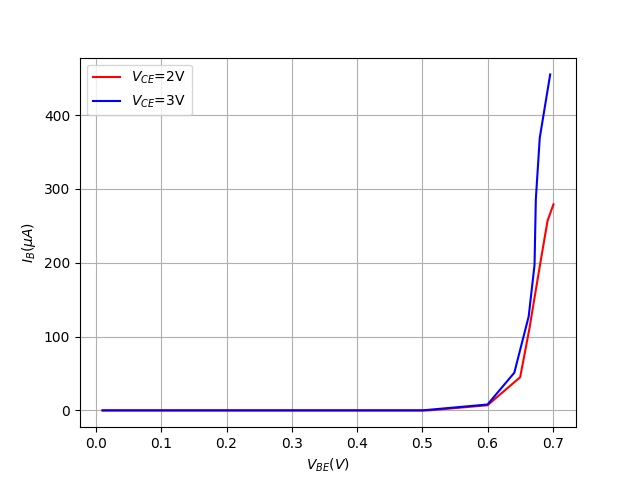
\includegraphics[width=0.8\textwidth]{D:/ronit/IISER-K/6 SEM/PH3204/Reports/exp02/plot1.png}  % Path to your image file
    \caption{Input characteristics of BJT for $V_{CE}=2V$ and $V_{CE}=3V$}  % Optional caption
    \label{fig:part01_01}  % Optional label for referencing
  \end{figure}\noindent
  Note that, although, it was expected that the curve for $V_{CE}=2V$ to be towards left of the curve corresponding to $V_{CE}=3V$,it is not so. This may be due to some error in the experiment.\\
\section{CE Output Characteristics}
We shall now study the output characteristics of a n-p-n transistor in CE configuration. We shall study the variation of $\mathrm{I_C}$ v/s $\mathrm{V_{CE}}$., keeping the base current $\mathrm{I_B}$ constant. We have carried out the experiment for $\mathrm{I_B}=10 \mu A$ and $\mathrm{I_B}=20 \mu A$ and $\mathrm{I_B}= 30 \mu A$. The data obtained has been tabulated below.
\begin{longtable}{|l|l|l|l|}
	\hline
    $\mathrm{I_{B}(\mu A)}$ & $\mathrm{V_{CC}(V)}$& $\mathrm{V_{CE}(mV)}$&  $\mathrm{I_{C}(\mu A)}$ \\ \hline
	\endfirsthead
	\hline
    $\mathrm{I_{B}(\mu A)}$ & $\mathrm{V_{CC}(V)}$ & $\mathrm{V_{CE}(mV)}$&  $\mathrm{I_{C}(\mu A)}$ \\ \hline
	\endhead
	\hline
	\endfoot
	\endlastfoot
    10  & 0.2  & 43   & 195  \\ \hline
    10  & 0.3  & 43   & 254  \\ \hline
    10  & 0.4  & 64   & 357  \\ \hline
    10  & 0.5  & 66   & 458  \\ \hline
    10  & 0.6  & 69   & 524  \\ \hline
    10  & 0.7  & 82   & 623  \\ \hline
    10  & 0.8  & 106  & 670  \\ \hline
    10  & 0.9  & 105  & 731  \\ \hline
    10  & 1.0  & 115  & 834  \\ \hline
    10  & 1.2  & 115  & 1018 \\ \hline
    10  & 1.5  & 189  & 1231 \\ \hline
    10  & 1.8  & 249  & 1430 \\ \hline
    10  & 2.0  & 359  & 1472 \\ \hline
    10  & 2.5  & 861  & 1473 \\ \hline
    10  & 3.0  & 1400 & 1470 \\ \hline
\caption{Table for Output characteristics for $\mathrm{I_B=10 \mu A}$}
\label{tab:part02_01}
\end{longtable}
\begin{longtable}{|l|l|l|l|}
	\hline
    $\mathrm{I_{B}(\mu A)}$ & $\mathrm{V_{CC}(V)}$ & $\mathrm{V_{CE}(mV)}$&  $\mathrm{I_{C}(\mu A)}$ \\ \hline
	\endfirsthead
	\hline
    $\mathrm{I_{B}(\mu A)}$ & $\mathrm{V_{CC}(V)}$& $\mathrm{V_{CE}(mV)}$&  $\mathrm{I_{C}(\mu A)}$ \\ \hline
	\endhead
	\hline
	\endfoot
	\endlastfoot
    20  & 0.1  & 15.6  & 73   \\ \hline
    20  & 0.2  & 23.8  & 184  \\ \hline
    20  & 0.3  & 30.9  & 229  \\ \hline
    20  & 0.4  & 39.7  & 336  \\ \hline
    20  & 0.5  & 44.2  & 422  \\ \hline
    20  & 0.6  & 49.0  & 493  \\ \hline
    20  & 0.7  & 47.9  & 582  \\ \hline
    20  & 0.8  & 53.4  & 720  \\ \hline
    20  & 0.9  & 64.4  & 810  \\ \hline
    20  & 1.0  & 65.9  & 840  \\ \hline
    20  & 1.2  & 70.1  & 1018 \\ \hline
    20  & 1.4  & 79.2  & 1250 \\ \hline
    20  & 1.6  & 83.5  & 1386 \\ \hline
    20  & 1.8  & 89.0  & 1555 \\ \hline
    20  & 2.0  & 102.8 & 1713 \\ \hline
    20  & 2.5  & 130.6 & 2390 \\ \hline
    20  & 3.0  & 290.0 & 2750 \\ \hline
    20  & 3.5  & 390.0 & 3110 \\ \hline
    20  & 4.0  & 957.0 & 3160 \\ \hline
    20  & 5.0  & 1855.0 & 3250 \\ \hline
\caption{Table for Output characteristics for $\mathrm{I_B=20 \mu A}$}
\label{tab:part02_02}
\end{longtable}
\begin{longtable}{|l|l|l|l|}
	\hline
    $\mathrm{I_{B}(\mu A)}$ & $\mathrm{V_{CC}(V)}$  & $\mathrm{V_{CE}(mV)}$&  $\mathrm{I_{C}(\mu A)}$ \\ \hline
	\endfirsthead
	\hline
    $\mathrm{I_{B}(\mu A)}$ & $\mathrm{V_{CC}(V)}$& $\mathrm{V_{CE}(mV)}$&  $\mathrm{I_{C}(\mu A)}$ \\ \hline
	\endhead
	\hline
	\endfoot
	\endlastfoot
    30  & 0.1  & 15.6  & 105  \\ \hline
    30  & 0.2  & 20.9  & 183  \\ \hline
    30  & 0.3  & 30.0  & 267  \\ \hline
    30  & 0.4  & 35.5  & 385  \\ \hline
    30  & 0.5  & 43.2  & 472  \\ \hline
    30  & 0.6  & 45.5  & 563  \\ \hline
    30  & 0.7  & 53.8  & 638  \\ \hline
    30  & 0.8  & 55.8  & 710  \\ \hline
    30  & 0.9  & 61.6  & 785  \\ \hline
    30  & 1.0  & 62.2  & 856  \\ \hline
    30  & 1.2  & 70.2  & 1026 \\ \hline
    30  & 1.5  & 81.9  & 1324 \\ \hline
    30  & 1.8  & 93.6  & 1503 \\ \hline
    30  & 2.0  & 98.6  & 1700 \\ \hline
    30  & 2.2  & 117.0 & 2130 \\ \hline
    30  & 2.4  & 127.9 & 2270 \\ \hline
    30  & 2.6  & 140.7 & 2520 \\ \hline
    30  & 2.8  & 153.7 & 2700 \\ \hline
    30  & 3.0  & 160.4 & 2830 \\ \hline
    30  & 3.5  & 190.1 & 3390 \\ \hline
    30  & 4.0  & 230.0 & 3890 \\ \hline
    30  & 5.0  & 510.0 & 4540 \\ \hline
    30  & 6.0  & 1500.0 & 4580 \\ \hline
\caption{Table for Output characteristics for $\mathrm{I_B=30 \mu A}$}
\label{tab:part02_03}
\end{longtable}
\begin{figure}[H]  
    \centering  
    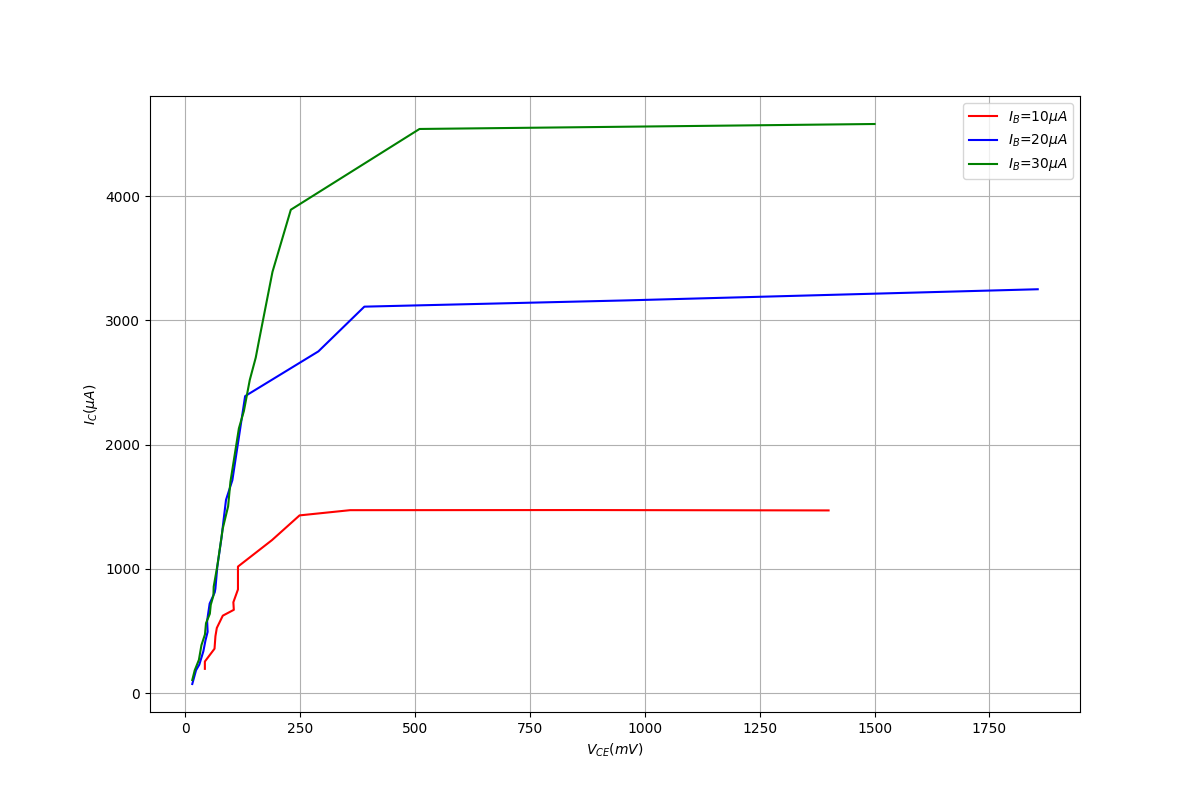
\includegraphics[width=0.8\textwidth]{D:/ronit/IISER-K/6 SEM/PH3204/Reports/exp02/plot2.png}  % Path to your image file
    \caption{Output characteristics of BJT for $I_{B}=10\mu A,20\mu A$ and $30\mu A$}  % Optional caption
    \label{fig:part01_02}  % Optional label for referencing
  \end{figure}\noindent
As expected, we observe from the graph that the output current $\mathrm{I_C}$ increases with the increase in the collector-emitter voltage $\mathrm{V_{CE}}$ for a constant base current $\mathrm{I_B}$.
\section{Conclusion}
In this experiment, we attempted to the study the input and output characteristics of a Bipolar Junction Transistor in CE mode. While verifying the input characteristics, we observed that , contrary to our expectations, the curve for $V_{CE}=2V$ was not towards the left of the curve for $V_{CE}=3V$. This may be due to some error in the experiment. \\
On the other hand, in output characteristics, we observed that the output current $\mathrm{I_C}$ increases with the increase in the collector-emitter voltage $\mathrm{V_{CE}}$ before reaching saturation for a fixed value of base current $\mathrm{I_B}$.\\
\\
Using, table \ref{tab:part02_01}, \ref{tab:part02_02} and \ref{tab:part02_03}, we can calculate the value of $\beta$ for the transistor using the formula $\beta = \frac{I_C}{I_B}$.
The value of $\beta$ for the transistor is found to be $147$, $162.5$ and $152.67$ for $\mathrm{I_B}=10 \mu A,20 \mu A$ and $30 \mu A$ respectively.
\section{Sources of Error}
\begin{itemize}
    \item The multimeter used for measuring of voltage and current may not be accurate.
    \item The connections may not be proper and transistor may not be in a proper condition. Also, the resistance of the wires may not be negligible.
    \item During a lot of readings, the values fluctuated a lot and could have given rise to errors.
\end{itemize}

 
\end{document}